\documentclass[10pt]{article}
\usepackage[polish]{babel}
\usepackage[utf8]{inputenc}
\usepackage[T1]{fontenc}
\usepackage{amsmath}
\usepackage{amsfonts}
\usepackage{amssymb}
\usepackage[version=4]{mhchem}
\usepackage{stmaryrd}
\usepackage{graphicx}
\usepackage[export]{adjustbox}
\graphicspath{ {./images/} }

\begin{document}
\begin{enumerate}
  \item Udowodnij, że jeżeli \(|a| \leq 1 \mathrm{i}|b| \leq 1\), to \(1-a b \geq|a-b|\)
  \item Rozwiąż w liczbach naturalnych równanie \(x^{2}+y^{2}=2020\)
  \item Niech \(A^{\prime}, B^{\prime}, C^{\prime}\) będą spodkami wysokości trójkąta ABC. Trójkąt \(A^{\prime} B^{\prime} C^{\prime}\) nazywamy trójkątem spodkowym trójkąta \(A B C\). Udowodnij, że pole trójkąta można obliczyć mnożąc promień okręgu opisanego przez połowę obwodu trójkąta spodkowego.\\
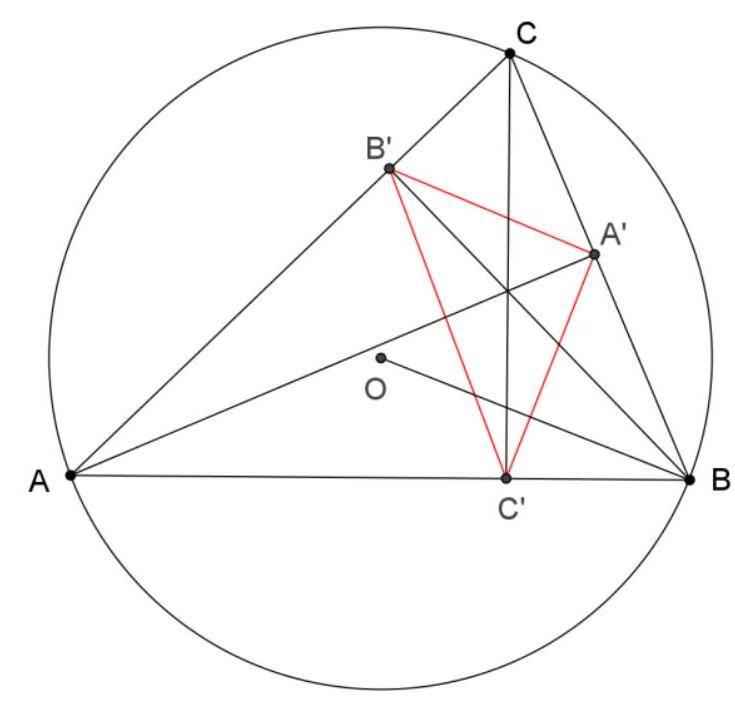
\includegraphics[max width=\textwidth, center]{2024_11_21_e1a346b5162485125e83g-1}
\end{enumerate}

\end{document}